\documentclass[12pt,a4paper]{report}
\usepackage[utf8]{inputenc}
\usepackage[english]{babel}
\usepackage[T1]{fontenc}
\usepackage{amsmath}
\usepackage{amsfonts}
\usepackage{amssymb}
\usepackage{lmodern}
\usepackage{courier}
\usepackage[none]{hyphenat}
\usepackage{authoraftertitle}
\usepackage[final]{graphicx}
\DeclareGraphicsExtensions{.pdf,.png,.jpg}
\usepackage{geometry}
\geometry{a4paper, top=30mm, left=25mm, right=25mm, bottom=30mm, headsep=10mm, footskip=12mm}
\usepackage{color}
\usepackage{hyperref}
\usepackage[tikz]{bclogo}

\hypersetup{
	colorlinks=true,
	linkcolor=black,
	urlcolor=red,
	citecolor=black,
	linktoc=all
}

\usepackage{listings}
\definecolor{forestgreen}{RGB}{34,139,34}
\definecolor{orangered}{RGB}{239,134,64}
\definecolor{darkblue}{rgb}{0.0,0.0,0.6}
\definecolor{gray}{rgb}{0.4,0.4,0.4}
\definecolor{pblue}{rgb}{0.13,0.13,1}
\definecolor{pgreen}{rgb}{0,0.5,0}
\definecolor{pred}{rgb}{0.9,0,0}
\definecolor{pgrey}{rgb}{0.46,0.45,0.48}

\lstdefinestyle{XML} {
	language=XML,
	extendedchars=true, 
	breaklines=true,
	breakatwhitespace=true,
	emph={},
	emphstyle=\color{red},
	basicstyle=\ttfamily,
	columns=fullflexible,
	commentstyle=\color{gray}\upshape,
	morestring=[b]",
	morecomment=[s]{<?}{?>},
	morecomment=[s][\color{forestgreen}]{<!--}{-->},
	keywordstyle=\color{orangered},
	stringstyle=\ttfamily\color{black}\normalfont,
	tagstyle=\color{darkblue}\bf,
	morekeywords={attribute,xmlns,version,type,release},
	otherkeywords={attribute=, xmlns=},
	basicstyle=\ttfamily\scriptsize
}

\lstdefinestyle{Java} {
	language=Java,
	showspaces=false,
	showtabs=false,
	breaklines=true,
	showstringspaces=false,
	breakatwhitespace=true,
	commentstyle=\color{pgreen},
	keywordstyle=\color{pblue},
	stringstyle=\color{pred},
	basicstyle=\ttfamily,
	moredelim=[il][\textcolor{pgrey}]{$$},
	moredelim=[is][\textcolor{pgrey}]{\%\%}{\%\%}
}


%Header & Footer
%\usepackage{lastpage}
%\rfoot{\thepage\ of \pageref{LastPage}}



\date{\today}
\author{Ari Ayvazyan}
\title{JEE Security}

\begin{document}

\maketitle
\tableofcontents


\chapter{Secure Systems}
\section{Aspects of Security}
The most important aspects of security form the so called \textbf{CIA-triad}.

\begin{itemize}
\item Confidentiality
\item Integrity
\item Availability
\end{itemize}

Another important aspect, that is not included within CIA, is \textbf{Non-Repudiation}.

\subsection{Confidentiality}
For secure systems it normally is very important that data cannot be read by unauthorized users, neither when stored in it's storage location nor during transmission.

\subsection{Integrity}
For secure systems it normally is very important that data and the state of the system cannot be modified by unauthorized users. In most cases, integrity also includes that only changes that are compliant to rules can be made.\\
Integrity issues are especially dangerous because they can lead to an undefined system state.

\subsection{Availability}
The availability of a system describes how stable the system is against error conditions and how available it is in general.

\subsection{Non-Repudiation}
Non-Repudiation means that actions can only be executed by their defined identities (eg. user groups).\\
This way it is possible to make users accountable for their actions.

\chapter{JEE Security Structure}
\section{Introduction to Security Architecture}
Most web applications have a few things in common:\\
They need to figure out who is the user that is using the application and what is he allowed to do and see.\\\\
A typical application has more than one security layer, it may be protected by only being available from a specified network or VPN. In addition there usually is some kind of identity determination followed by a SQL user with permission to query only the required functions and data sets.\\
On top of this, there should be output escaping to ensure that a attacker, who is able to manipulate the output for other users, is limited in the harm he is able to cause.\\
\begin{figure}[h]
\centering
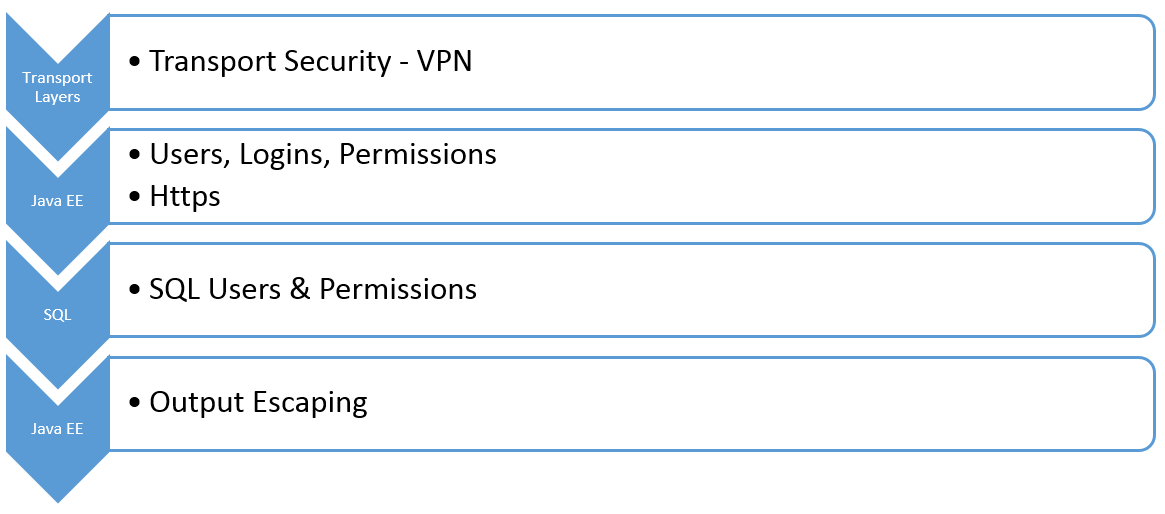
\includegraphics[width=1\linewidth]{res/SecurityLayers}
\caption{Security Layers in a common JEE application}
\label{fig:SecurityLayers}
\end{figure}
\newpage \noindent
According to Oracle\cite{oracleDoc}, there are two ways to implement such access control functionality with Java EE:
\begin{enumerate}
	\item Declarative Security (this includes Annotations and XML-Files)\\
	is applied during the application's deployment.
	\item Programmatic Security\\
	is applied by the application itself at runtime.
\end{enumerate}
While the programmatic implementation offers a wider range of customization, the declarative provides a well structured and easy to use approach.\\

\chapter{Authentication \& Authorization}
\section{Authentication}
Authentication describes the identification process. This is mostly done by asking for a user-name \& password or sending a Token/Hash.

\section{Authorization}
Authorization is what happens after you are authenticated.\\
It deals with the question of what a authenticated person is allowed to do.\\
Authorization may be applied to URLs or resources like Beans and Servlets.\\

\begin{figure}[h]
	\centering
	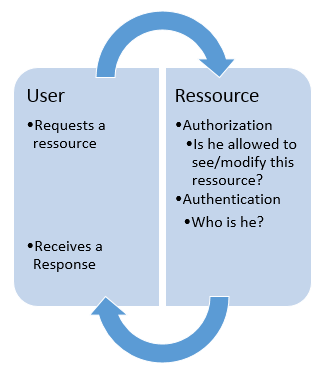
\includegraphics[width=0.5\linewidth]{res/AuthenAuthor}
	\caption{Authentication \& Authorization}
	\label{fig:AuthenAuthor}
\end{figure}

\section{Principals}
A Principal is an identity that can be authenticated.\\
E.g. a Unique user name\\
Principals are handled by the container and need to be configured there. This includes storage and queries\\

\section{Credential}
A Credential is defined as information that is used to authenticate a Principal.\\
E.g. a Password\\
Credentials are just like Principals handled by the container.

\section{Groups}
Groups and Principals can be mapped together. This information is handled by the container and by that not accessible by the application. To make this information available to the server, Groups can be mapped to Roles.\\
Group-Role mappings are usually defined in the (vendor-specific).xml file.\\

\section{Roles}
A Role is a abstract layer in front of the container that can be accessed application wide, they are declared in the web.xml file\\
Roles can be mapped to Principals and Groups via the (vendor-specific).xml file.\\

\section{Realms}
Realms are also known as Security policy domains, they store and provide information about Principals, their Credentials and their Groups.\\
A Realm may take use of a database, a file structure, a connection to a service...\\\\
Realms are handled by the container, some come with pre-configured realms.

\chapter{Deployment Descriptors}
A Deployment Descriptor describes how a Java EE application should be deployed.\\
They contain information about security constraints, accessibility and resource references.\\\\
Deployment Descriptors are XML-Files that are by default located in the /WEB-INF/ directory.\\
The following deployment descriptors may be found here:
\begin{itemize}
	\item web.xml
	\item <vendor-specific>.xml (E.g. when using Glassfish: glassfish-web.xml)
\end{itemize}

\section{web.xml}
The Web.xml file stores apart from usual deployment information like servlet mappings also security related information about:\\
\begin{itemize}
	\item Protected Resources
	\item Security Roles
	\item Authentication methods
\end{itemize}
The following XML snippets are located within the <web-app></web-app> tag.

\subsection*{Protected Resources}
It is possible to limit access to resources by defining a security constraint on the URL or by securing the resource itself.\\
E.g. to protect the /primes/ URL with all its subdirectories we would have to use the following code:\\
\begin{bclogo}[couleur=yellow!15,arrondi=0.1,logo=\bccrayon, ombre = true]{Securing a URL}
\begin{lstlisting}[style=XML]
<security-constraint>
	<web-resource-collection>
		<web-resource-name>primes
		</web-resource-name>
<!--Include /primes/ including all following subfolders-->
		<url-pattern>/primes/*</url-pattern>
<!-- This would result in a security leak because 
	there are more http-methods than GET and POST-->
<!-- by defining no http-method at all, 
	everything will be blocked-->
		<http-method>GET</http-method>
		<http-method>POST</http-method>
	</web-resource-collection>
	
	<auth-constraint>
		<role-name>view_role</role-name>
	</auth-constraint>
</security-constraint>
\end{lstlisting}
\end{bclogo}
In result, only a user with the role view\_role is allowed to access the defined resources.

\subsection*{Security Roles}
A Security Role was used in the last subsection "Protected Resources", we declared that only users with the role "view\_role" are allowed to view the restricted URL.\\
A Security Role is a abstract layer in front of the container, it defines a identifier which we can use for constraints. This identifier is then used by the container to specify its meaning by telling who is part of this Security Role.\\
\begin{bclogo}[couleur=yellow!15,arrondi=0.1,logo=\bccrayon, ombre = true]{Defining a Security Role}
\begin{lstlisting}[style=XML]
    <security-role>
	    <description>This role has view access</description>
	    <role-name>view_role</role-name>
    </security-role>
\end{lstlisting}
\end{bclogo}
\subsection*{Authentication Methods}
There are several kinds of Authentication Methods with different security behaviors.\\
BASIC Authentication opens a login prompt when a user tries to access the secured URL, it is simple to implement but insecure. BASIC Authentication sends the user's credentials unencrypted to the server.\\
\begin{bclogo}[couleur=yellow!15,arrondi=0.1,logo=\bccrayon, ombre = true]{Defining BASIC Authentication}
\begin{lstlisting}[style=XML]
    <login-config>
	    <auth-method>BASIC</auth-method>
	    <realm-name>Java EE Login</realm-name>
    </login-config>
\end{lstlisting}
\end{bclogo}

\section{(vendor-specific).xml}
Most containers use in addition to the web.xml a vendor specific XML file that is usually located in the same directory with web.xml.\\
E.g. Glassfish calls this file "glassfish-web.xml" while Tomcat has named it "context.xml".\\\\
The following settings can be configured there:\\
\begin{itemize}
	\item Principal – Role Mapping
	\item Group – Role Mapping
	\item Other container specific configuration.
\end{itemize}

\subsection{User Role Mapping}
It is possible to Map Users (Principals) to Roles. This setting is container dependent.\\
\begin{bclogo}[couleur=yellow!15,arrondi=0.1,logo=\bccrayon, ombre = true]{Principal mapping with Glassfish}
	\begin{lstlisting}[style=XML]
	<glassfish-web-app>
	<security-role-mapping>
		<role-name>view_role</role-name>
		<principal-name>Blitzmann</principal-name>
	</security-role-mapping>
	</glassfish-web-app>
	\end{lstlisting}
\end{bclogo}
This setting maps the user "Blitzmann" to the role "view\_role".

\subsection{Group Role Mapping}
It is possible to Map Users (Principals) to Roles. This setting is container dependent.\\
\begin{bclogo}[couleur=yellow!15,arrondi=0.1,logo=\bccrayon, ombre = true]{Principal mapping with Glassfish}
	\begin{lstlisting}[style=XML]
	<glassfish-web-app>
	<security-role-mapping>
	<role-name>view_role</role-name>
	<group-name>view_group</group-name>
	</security-role-mapping>
	</glassfish-web-app>
	\end{lstlisting}
\end{bclogo}
This setting maps the group "view\_group" to the role "view\_role".

\chapter{Implementation Sample}
The following sample may be found at this URL:\\
\href{https://github.com/aayvazyan-tgm/JavaEESecurityExample}{https://github.com/aayvazyan-tgm/JavaEESecurityExample}\\
\section{Objective}
The objective of our sample is to deny access to our service, that is reachable at .../primes/, to everybody except users that are granted permission by possessing the "view\_role" role.
\begin{figure}[h!]
\centering
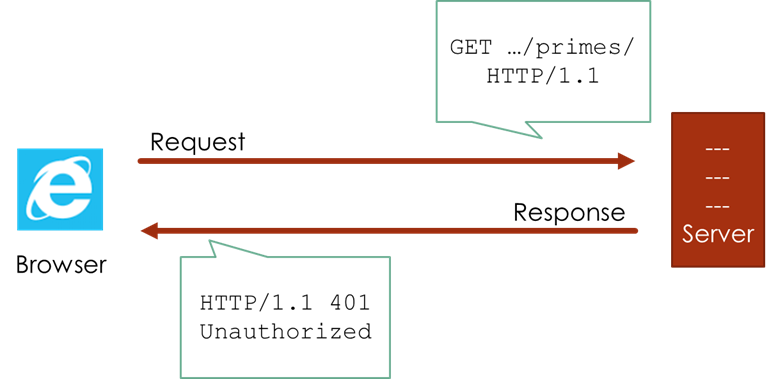
\includegraphics[width=1\linewidth]{res/Unauthorized}
\caption{The user tries to access a resource without authentication}
\label{fig:Unauthorized}
\end{figure}

\noindent
To figure out which user possesses the "view\_role" role, we first have to authenticate the user. This shall happen with a login promt. After transmitting the credentials to the server and having the correct role, the user should be able to access the resource.
\begin{figure}[h!]
	\centering
	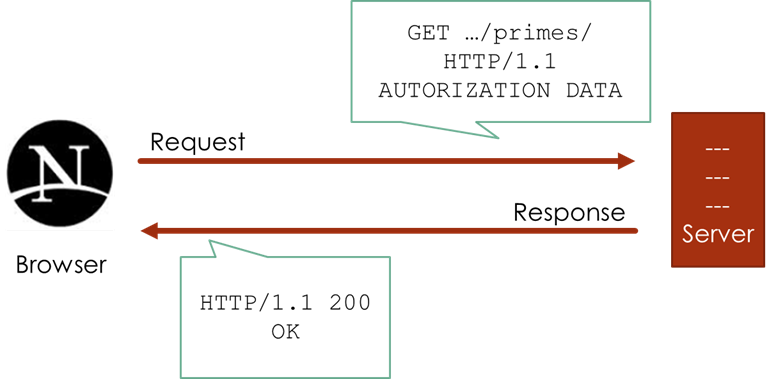
\includegraphics[width=1\linewidth]{res/Authorized}
	\caption{The user sends authentication data with his request}
	\label{fig:Authorized}
\end{figure}

\section{Setup}
A Glassfish server is used as the container.\\
The user "Blitzmann" was created by navigating to the GlassFish Server Administration Console, then to Configuration -> server-config -> Security -> Realms -> file -> add Property and entering "Blitzmann" as Name and the desired password as Value.\\
The rest is configured in the web.xml and glassfish-web.xml
\begin{bclogo}[couleur=yellow!15,arrondi=0.1,logo=\bccrayon, ombre = true]{web.xml}
	\begin{lstlisting}[style=XML]
    <security-constraint>
    <web-resource-collection>
	    <web-resource-name>primes</web-resource-name>
	    <!--Include all urls that are starting with /primes/ -->
	    <url-pattern>/primes/*</url-pattern>
	    <!-- This would result in a security leak because 
		    there are more http-methods than get and post-->
	    <!-- by defining no http-method at all 
		    everything will be blocked-->
	    <!--http-method>GET</http-method>
	    <http-method>POST</http-method-->
    </web-resource-collection>
	    <auth-constraint>
		    <role-name>view_role</role-name>
	    </auth-constraint>
    </security-constraint>
    
    <login-config>
	    <auth-method>BASIC</auth-method>
	    <realm-name>file</realm-name>
    </login-config>
    
    <security-role>
        <description>This role has view access</description>
        <role-name>view_role</role-name>
    </security-role>
	\end{lstlisting}
\end{bclogo}
\begin{bclogo}[couleur=yellow!15,arrondi=0.1,logo=\bccrayon, ombre = true]{glassfish-web.xml}
	\begin{lstlisting}[style=XML]
	<glassfish-web-app>
		<security-role-mapping>
			<role-name>view_role</role-name>
			<group-name>view_group</group-name>
			<principal-name>Blitzmann</principal-name>
		</security-role-mapping>
	</glassfish-web-app>
	\end{lstlisting}
\end{bclogo}

\chapter{Security with Enterprise Beans}
Enterprise Java Beans offers many different options to secure your application. Enterprise Java Beans can fully organize both Transactions and Authorization.

\section{Authentication and User Groups}
Enterprise Java Beans offers role-based authentication to limit the usage of certain components. This includes whole Beans, single methods independent of their signature and methods with a definition of their signature.
Roles and permissions for Enterprise Java Beans are normally defined in the deployment descriptor. Details on how to define roles and authentication can be found in chapter 1.4.1.

\section{Permissions}
Method access permissions are defined as following:

\subsection{<method permission>}
Access definition based on roles.

\subsection{<unchecked>}
The container activates a method unchecked.

\subsection{<exclude-list>}
The method cannot be called.

\section{Security context}
Enterprise Java beans offers the option to pass the security identity of a caller within the security context. It is both possible to pass the identity either untouched or to change the security identity with the call. This can be set within the <security-identity> element in the deployment-descriptor.

\subsection{Passing the identity}
\begin{bclogo}[couleur=yellow!15,arrondi=0.1,logo=\bccrayon, ombre = true]{web.xml}
\begin{lstlisting}[style=XML]
<security-identity>
<use-caller-identity></use-caller-identity>
</security-identity>
\end{lstlisting}
\end{bclogo}

\subsection{Changing the identity}
\begin{bclogo}[couleur=yellow!15,arrondi=0.1,logo=\bccrayon, ombre = true]{web.xml}
\begin{lstlisting}[style=XML]
<security-identity>
<run-as>
<description>Info from assembler to deployer</description>
<role-name>Admin</role-name>
</run-as>
</security-identity>
\end{lstlisting}
\end{bclogo}
It is crucial that the role defined in the <run-as> can be resolved to a user. The assembler has to use an existing logic role or define a new one that must then be mapped to a concrete user.
Both assembler and deployer have to pay attention that no changes can happen to the security identity during a running transaction.

\section{Security with Annotations}
A different way to define and use roles in Enterprise Java Beans is using annotations direcly in the source code.

\subsection{@DeclareRoles}
Indicates that class will accept those declared roles. Annotations are applied at class level.

\subsection{@RolesAllowed}
Indicates that a method can be accessed by user of role specified. Can be applied at class level resulting which all methods of class can be accessed buy user of role specified. 

\subsection{@PermitAll}
Indicates that business method is accessible to all. Can be applied at class as well as at method level. 

\subsection{@DenyAll}
Indicates that business method is not accessible to any of user specified at class or at method level.

\subsection{Example}

\begin{bclogo}[couleur=yellow!15,arrondi=0.1,logo=\bccrayon, ombre = true]{SecuredBean.java}
\begin{lstlisting}[style=Java]
@Stateless
@DeclareRoles({"Autoren", "Lektoren"})
public class SecuredBean implements SecuredRemote {
	@PermitAll
	public boolean ckeck(){ ... }
	
	@RolesAllowed("Autoren")
	public boolean deposit(double amount) { ... }
	
	@DenyAll
	public boolean kill() { ... }
}
\end{lstlisting}
\end{bclogo}
[6, Enterprise Java Beans, Page 328: EJB-Sicherheit]

\section{Programmatic}
Even though the Enterprise Java Beans documentation recommends using programmatic security management “only in the less frequent situations” and rather use the security management offered by the Enterprise Java Beans container, there are certain situations where declarative security management is too static and not flexible enough. Further, Enterprise Java Beans offers an Interface that allows to place security queries directly into the Bean-code.
This is established by the Enterprise Java Beans context object named SessionContext or respectively EntityContext.

\subsection{getCallerPrincipal()}
Returns the current principal (caller). It returns an object of the type java.security.Principal. Using its getName() method will return the name of the current principal.
This method could for example be used if a Bean-method should access a database using the name of the principal as search term

\subsection{isCallerInRole(<param>)}
Returns if the current principal has a certain role. It can be used to make further security checks within the Bean-class that cannot be done declaratively, or are very hard to implement using access permissions.
Before it is possible to use this method a Bean-developer has to declare a role reference in the deployment-descriptor. This reference has to represent the value of the call isCallerinRole(String role). This value will be linked with a logic role at deployment. A role reference is created using a <security-role-ref> element.

\subsection{Attention}
Both those methods are only allowed to be called within a Bean-instance for which the container can offer the security context of a client.

\subsection{Example}
\begin{bclogo}[couleur=yellow!15,arrondi=0.1,logo=\bccrayon, ombre = true]{SecuredBean.java}
\begin{lstlisting}[style=Java]
public void getTextUpd() {
	// erhalte den Anwendername aus ctx
	// (der EJBContext wurde in der
	// Instanzenvariablen ctx gespeichert)
	String userName =
	ctx.getCallerPrincipal().getName();
	// teste die Rolle des Aufrufers:
	if (ctx.isCallerInRole("Autor")) {
		
		//z.B. Zugriff auf DB-Saetze
		//mit Schluessel = "userName"
		...
	}
	else{
		//Zugriff protokollieren
		System.out.println("nicht autorisierter
		Zugriff von Anwender: " + userName);
	}
}
\end{lstlisting}
\end{bclogo}

[6, Enterprise Java Beans, Page 335: EJB-Sicherheit]


\chapter{Securing Application Clients}
\section{General}
In general, when developing a Java EE application client a lot of security concerns that you would have with any normal application occur here as well.\\

This includes but is not limited to:
\begin{itemize}
\item Decompiling
\item Malware
\item Disassembling
\end{itemize}
This means you want to keep the amount of programmatic security management as low as possible and be careful with confidential data.\\\\

The basic protection precautions of secure programming in Java are:

\begin{itemize}
\item Deliberate use of privileged code
\item Appropriate definition of static fields
\item Reduction of visibility
\item Package safety
\item Immutable objects
\item Serialization
\item Native methods
\item Dealing carefully with confidential data in the heap
\end{itemize}

\section{Java EE Application Clients}
When developing Java EE application clients you can avoid a lot of client security leaks by reducing the "thickness" of the client. Never forget that an attacker could potentially write his own application client! Therefore, Java EE authentication requirements for application clients are the same as for other Java EE components, and the same authentication techniques can be used as for other Java EE application components. This means it is not possible to write an application client to bypass a web-clients authentication requirement. Unprotected web resources can still be accessed without authentication.

\section{Authentication}
When accessing protected web resources, the usual varieties of authentication can be used: HTTP basic authentication (more details can be found in 1.4.1 Authentication), HTTP login-form authentication, or SSL client authentication.
Authentication is required when accessing protected enterprise beans. The authentication mechanisms available for enterprise beans are discussed in the chapter “Security with Enterprise Beans”.

\section{Login Modules}
An application client can use the Java Authentication and Authorization Service (JAAS) to create login modules for authentication.
To do this, write a class that implements the javax.security.auth.callback.CallbackHandler interface so that it can interact with users to enter specific authentication data, such as user names or passwords, or to display error and warning messages.
“Applications implement the CallbackHandler interface and pass it to the login context, which forwards it directly to the underlying login modules. A login module uses the callback handler both to gather input, such as a password or smart card PIN, from users and to supply information, such as status information, to users. Because the application specifies the callback handler, an underlying login module can remain independent of the various ways applications interact with users.” [3, Java EE 6 Documentation, Using Login Modules]

\section{Programmatic Login}
Programmatic login enables the client code to supply user credentials. If you are using an EJB client, you can use the com.sun.appserv.security.ProgrammaticLogin class with its convenient login and logout methods. Programmatic login is specific to a server. If possible, login modules should be preferred. 


\chapter{Working with Digital Certificates}
\section{Server Authentication}
\subsection{Signed by Certificate Authority}
Sometimes it is important to prove to your clients that you are who you claim to be.\\
This way it is easier for the client to detect phishing and other scamming attempts.\\

"It may be useful to think of a certificate as a “digital driver’s license” for an Internet address. The certificate states with which company the site is associated, along with some basic contact information about the site owner or administrator." [3, Java EE 6 Documentation, Working with Digital Certificates]\\\\
If you want to run a site involved in e-commerce or in any other business environment in which authentication of identity is very important, you can purchase a certificate from a well-known certificate authority (CA) such as VeriSign or Thawte.

\subsection{Self-Signed}
Sometimes, it is not that important to prove who you are.
An administrator might simply want to ensure that data being transmitted and received by the server is private and cannot be intercepted by anyone listening on the connection. As obtaining CA certificates can be very time consuming and be quite expensive, in such cases, using a self-signed certificate can be a simpler alternative.

\section{HTTPS}
HTTP uses digital certificates to authenticate web clients. The HTTPS service of most web servers will not run unless a digital certificate has been installed.

\section{SSL}
Before it is possible to use the Secure Sockets Layer (SSL), an application or web server must have an associated certificate for each external interface (for example an IP Address) that accepts secure connections. The theory behind this design is that a server should provide some kind of reasonable assurance that its owner is who you think it is, particularly before receiving any sensitive information.

\section{Glassfish}
If you are using the GlassFish Server digital certificates have already been installed. These can be found in the domain-dir/config/ directory and are meant for development environments. For production purposes, you should generate your own certificates and have them signed by a CA if required.

\subsection{keystore.jks}
Stores the server certificate.

\subsection{cacerts.jks}
Contains all the trusted certificates, including client certificates.

\section{keytool}
One tool that can be used to set up a digital certificate is keytool, a key and certificate management utility that ships with the JDK. This tool enables users to administer their own public/private key pairs and associated certificates for use in self-authentication, whereby the user authenticates himself or herself to other users or services, or data integrity and authentication services, using digital 

\chapter{Output Escaping}
Security vulnerabilities happen to be found in the best applications, it is important to have more layers of security that prevent attackers from reading or modifying sensitive information.\\
E.g. we have a guestbook, everybody is allowed to write a entry. To prevent a attacker from writing custom HTML into our site, we may use input escaping. But if the attacker has managed to someway access our database in a different way, where no input escaping is applied, he would be able to perform his attack on our users.\\
To prevent him from doing so, we have to check our output (Output Escaping). This means that we only allow data to be passed that makes sense, so we do not allow HTML elements in this case.\\
It is important to use a framework to do so, they are proven to work, tested and can even save working hours.

\chapter{Frameworks}
\section{Shiro}
Offers: Authentication, Authorization, Cryptography\\
Simple to use\\\\

\section{Spring}
Offers: Authentication, Authorization, Cryptography\\
Very structured\\\\

\section{JAAS - Java Authentication and Authorization Service}
Offers: Authentication, Authorization, Cryptography\\
Included in Java SE since Java 1.4 (javax.security.auth)\\\\

\newpage
\begin{thebibliography}{99}
\bibitem{jSecVvulnerabilities}Java Security: Sicherheitslücken identifizieren und vermeiden, \\
Marc Schönefeld, 1. edition 2011\\
Publisher: Hüthig Jehle Rehm GmbH, Heidelberg. \\
ISBN/ISSN 978-3-8266-9105-8
\bibitem{EJSec}Enterprise Java Security: Building Secure J2EE Applications,\\
Marco Pistoia, Nataraj Nagaratnam, Larry Koved, Anthony Nadalin,\\
1. edition 2004 \\
Publisher: Addison-Wesley Professional.\\
ISBN/ISSN: ISBN 0-321-11889-8
\bibitem{oracleDoc}Official JavaEE Documentation, Oracle,\\
29.09.2014
http://docs.oracle.com/javaee/7/tutorial/partsecurity.htm\#GIJRP
Java EE 6,\\
Dirk Weil, 1. edition 2012\\
Publisher: entwickler.press\\
ISBN 978-3-86802-077-9
\bibitem{jeecookbook}Java EE 6 Cookbook for Securing, Tuning, and Extending Enterprise Applications,\\
Mick Knutson,\\
1. edition June 2012 \\
Publisher: Addison-Wesley Professional.\\
ISBN/ISSN: ISBN 9781849683166
\bibitem{JavaOne}JavaOne 2014: The Anatomy of a Secure Web Application Using Java, \\
Shawn McKinney \& John Field, September 29, 2014\\
San Francisco

\bibitem{EJB3}Enterprise JavaBeans 3.0, Grundlagen - Konzepte - Praxis\\
Martin Backschat \& Bernd Rücker\\
2. edition 2007\\
Publisher: Spektrum Akademischer Verlag
ISBN 978-3-8274-1510-3

\newpage
\listoffigures
\end{thebibliography}
\end{document}
